\documentclass[hyperref,]{ctexart}
\usepackage{lmodern}
\usepackage{amssymb,amsmath}
\usepackage{ifxetex,ifluatex}
\usepackage{fixltx2e} % provides \textsubscript
\ifnum 0\ifxetex 1\fi\ifluatex 1\fi=0 % if pdftex
  \usepackage[T1]{fontenc}
  \usepackage[utf8]{inputenc}
\else % if luatex or xelatex
  \ifxetex
    \usepackage{xltxtra,xunicode}
  \else
    \usepackage{fontspec}
  \fi
  \defaultfontfeatures{Mapping=tex-text,Scale=MatchLowercase}
  \newcommand{\euro}{€}
\fi
% use upquote if available, for straight quotes in verbatim environments
\IfFileExists{upquote.sty}{\usepackage{upquote}}{}
% use microtype if available
\IfFileExists{microtype.sty}{%
\usepackage{microtype}
\UseMicrotypeSet[protrusion]{basicmath} % disable protrusion for tt fonts
}{}
\ifxetex
  \usepackage[setpagesize=false, % page size defined by xetex
              unicode=false, % unicode breaks when used with xetex
              xetex]{hyperref}
\else
  \usepackage[unicode=true]{hyperref}
\fi
\usepackage[usenames,dvipsnames]{color}
\hypersetup{breaklinks=true,
            bookmarks=true,
            pdfauthor={蓝海; 彭莉},
            pdftitle={分析王培-技术报告},
            colorlinks=true,
            citecolor=blue,
            urlcolor=blue,
            linkcolor=magenta,
            pdfborder={0 0 0}}
\urlstyle{same}  % don't use monospace font for urls
\usepackage{longtable,booktabs}
\usepackage{graphicx,grffile}
\makeatletter
\def\maxwidth{\ifdim\Gin@nat@width>\linewidth\linewidth\else\Gin@nat@width\fi}
\def\maxheight{\ifdim\Gin@nat@height>\textheight\textheight\else\Gin@nat@height\fi}
\makeatother
% Scale images if necessary, so that they will not overflow the page
% margins by default, and it is still possible to overwrite the defaults
% using explicit options in \includegraphics[width, height, ...]{}
\setkeys{Gin}{width=\maxwidth,height=\maxheight,keepaspectratio}
\setlength{\emergencystretch}{3em}  % prevent overfull lines
\providecommand{\tightlist}{%
  \setlength{\itemsep}{0pt}\setlength{\parskip}{0pt}}
\setcounter{secnumdepth}{5}

\title{分析王培-技术报告}
\author{蓝海 \and 彭莉}
\date{}

% Redefines (sub)paragraphs to behave more like sections
\ifx\paragraph\undefined\else
\let\oldparagraph\paragraph
\renewcommand{\paragraph}[1]{\oldparagraph{#1}\mbox{}}
\fi
\ifx\subparagraph\undefined\else
\let\oldsubparagraph\subparagraph
\renewcommand{\subparagraph}[1]{\oldsubparagraph{#1}\mbox{}}
\fi

\begin{document}
\maketitle

{
\setcounter{tocdepth}{2}
\tableofcontents
}
\section{业绩表现}

\subsection{王培}

自2007年7月至2009年6月任国泰君安证券研究所助理研究员,从事化工行业分析研究工作。自2009年7月至2016年2月任银河基金管理有限公司行业研究员、基金经理助理、投资副总监兼基金经理。2016年2月加入中欧基金管理有限公司,先后担任事业部负责人、投资经理等职务。

王培前后共管理过5个不同的基金产品,有些基金创设时间太短,不具备分析价值,所以我们重点的挑选了3只基金为代表进行分析。它们是银河成长混合、银河300成长分级和银河创新成长混合。

\subsection{业绩表现}\label{-1}

中欧行业成长混合是王培在中欧基金管理的产品,虽然宣布他为产品经理是最近的时期,但是我们依据内部渠道得知他管理该基金的开始是2016年1月8日。
虽然该基金创设之初要求不低于80\%的股票资产按照约定是投资于中小盘股,但是后来更改为不低于80\%非现金资产投资于成长性行业,而所谓成长性行业由定量和定性结合的指标决定,因此我们认为使用沪深300作为参照指标是合理的。但是在与沪深300比较之前与成长指数做一次对比也是有意义的。
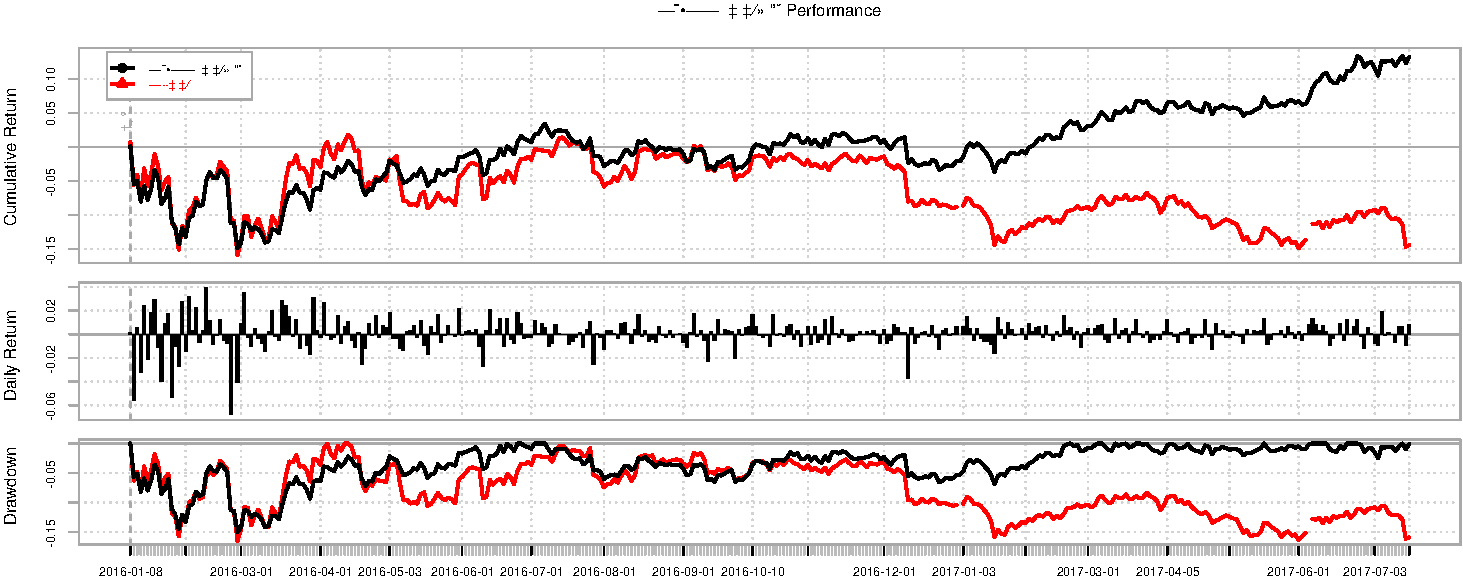
\includegraphics{wangpei-details_files/figure-latex/unnamed-chunk-2-1.pdf}

\begin{longtable}[]{@{}llclclc@{}}
\toprule
名称 & 最后半年 & 夏普率 & 一年 & 夏普率 & 两年 & 夏普率\tabularnewline
\midrule
\endhead
中欧行业成长混合 & 12.6\% & 2.1 & 12\% & 0.33 & 13\% &
0.25\tabularnewline
中创成长 & -7.2\% & -1.2 & -13\% & -0.52 & -14\% & -0.57\tabularnewline
\bottomrule
\end{longtable}

以下与沪深300比较:

\begin{figure}[htbp]
\centering
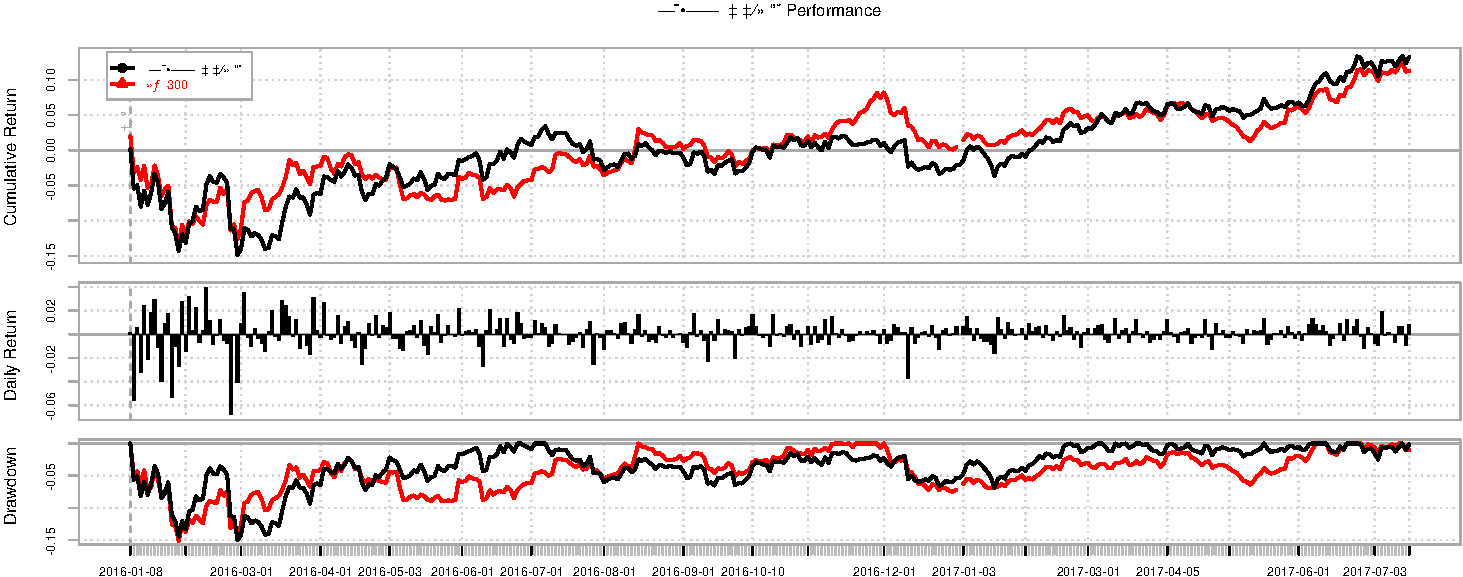
\includegraphics{wangpei-details_files/figure-latex/unnamed-chunk-3-1.pdf}
\caption{基金累计回报率与回撤}
\end{figure}

\begin{longtable}[]{@{}llclclc@{}}
\toprule
名称 & 最后半年 & 夏普率 & 一年 & 夏普率 & 两年 & 夏普率\tabularnewline
\midrule
\endhead
中欧行业成长混合 & 12.6\% & 2.1 & 12\% & 0.33 & 13\% &
0.25\tabularnewline
沪深300 & 8.9\% & 1.6 & 16\% & 0.28 & 11\% & 0.20\tabularnewline
\bottomrule
\end{longtable}

大多数时候该基金的业绩都没有跑过沪深300,但是我们要动态的看待这一现象。王培作为``成长新生代''里头的明星基金经理,在2015年股灾,市场风格有了根本的改变的时候,如何适应市场的变化,如何调整和丰富自己的投资体系是一个复杂的过程。在股灾后到入职中欧基金之前,王培的选股投资依旧还是原来的成长股风格,严重的不适应市场情形,其2015年5月接手的银河主题混合基金,在其离职之前的9个月的管理期内下跌了37.7\%。而入职中欧基金后,在他的投资范围内渐渐出现了茅台、五粮液、美的、上汽等传统大盘股。同时他原本擅长的成长股中也陆续挖掘出欧菲光、曲美家居等股票。所以尽管目前看来他的管理业绩没有超出沪深300,但是有从2017年1月以来其基金表现实际强于沪深300,在累计收益有一追赶弥补前期差距呢的过程。这充分显示一个善于学习勇敢转变的基金经理其未来是值得期待的。

\begin{figure}[htbp]
\centering
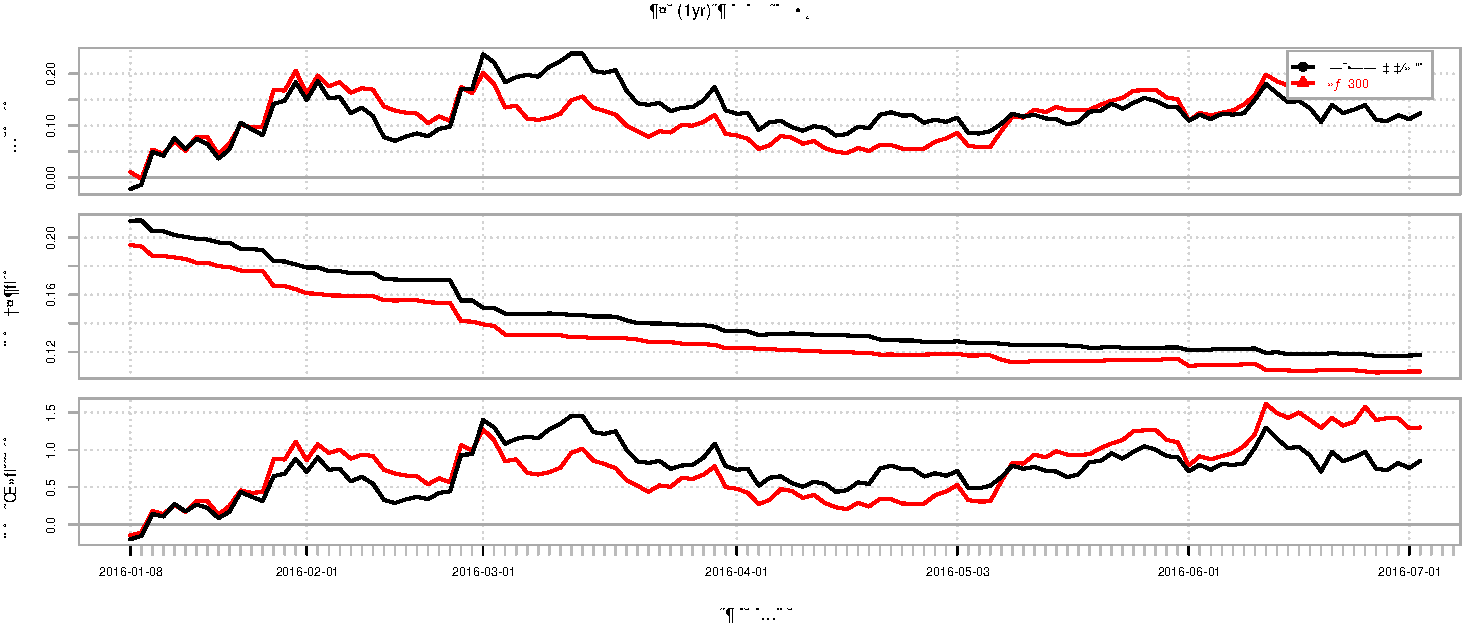
\includegraphics{wangpei-details_files/figure-latex/unnamed-chunk-4-1.pdf}
\caption{投资者收益风险比较}
\end{figure}

\subsection{历史表现}

\begin{figure}[htbp]
\centering
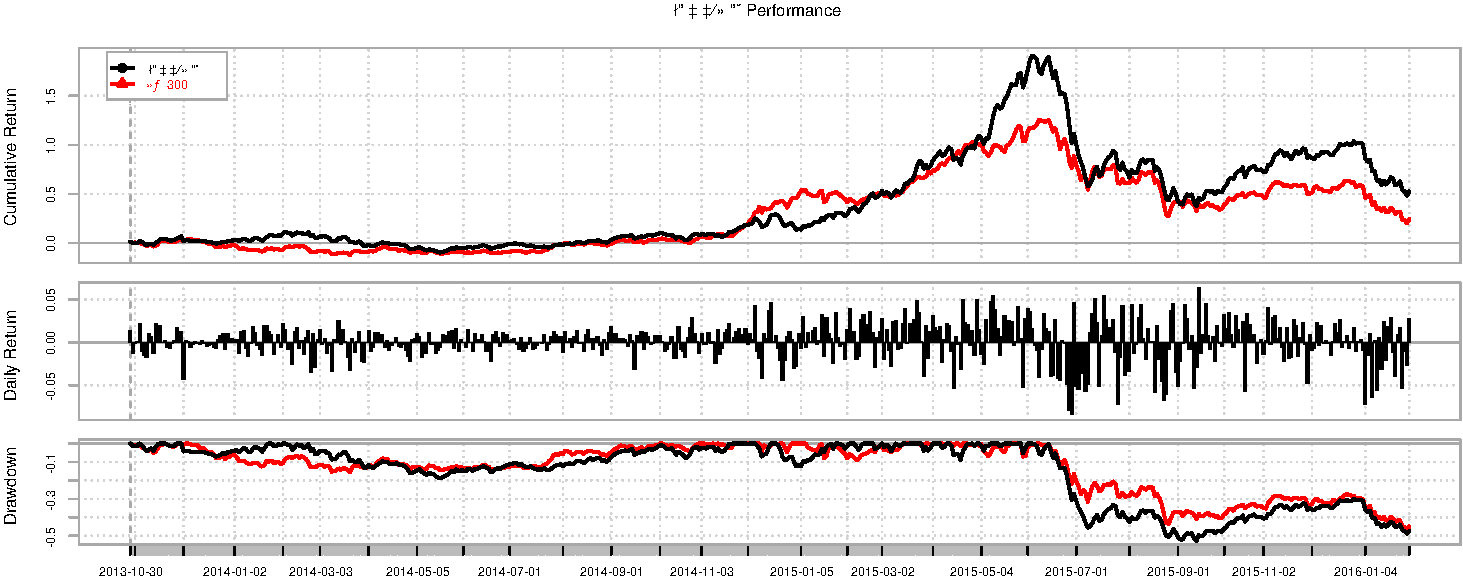
\includegraphics{wangpei-details_files/figure-latex/unnamed-chunk-5-1.pdf}
\caption{基金累计回报率与回撤}
\end{figure}

\begin{longtable}[]{@{}llclclc@{}}
\toprule
名称 & 最后半年 & 夏普率 & 一年 & 夏普率 & 两年 & 夏普率\tabularnewline
\midrule
\endhead
银河成长混合 & -20\% & -0.87 & 21\% & 0.52 & 53\% & 0.48\tabularnewline
沪深300 & -29\% & -1.24 & -19\% & 0.30 & 24\% & 0.20\tabularnewline
\bottomrule
\end{longtable}

\begin{figure}[htbp]
\centering
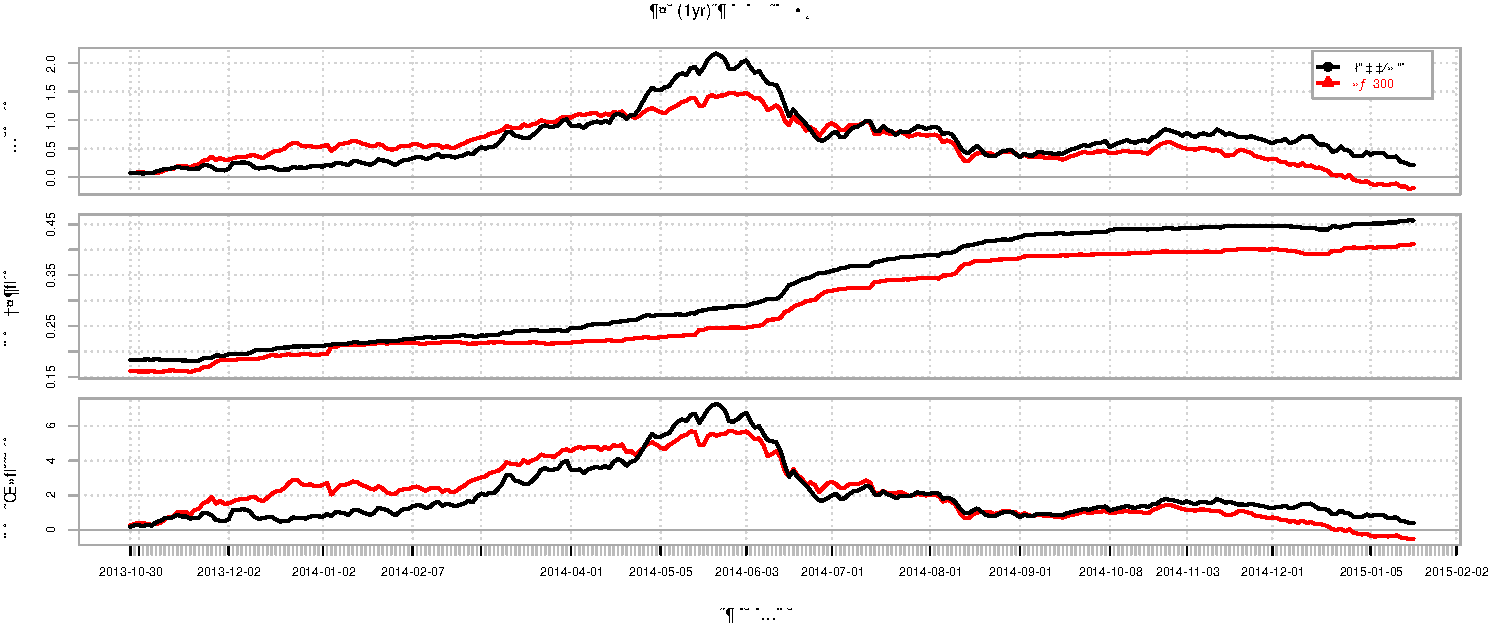
\includegraphics{wangpei-details_files/figure-latex/unnamed-chunk-6-1.pdf}
\caption{投资者收益风险比较}
\end{figure}

上图图清楚的表明自王培在管理银河成长混合基金以来相对于沪深300其累计收益率的表现以及面临的回撤。自2015年6月股灾发生以来的收益表现显示了管理者的风险控制能力的某种进化:从一开始大幅大于沪深300的回撤到后期二次、三次触底时回撤弧度缩小。当固定一年期的投资者,买入该基金与买入沪深300指数比较,大概只有一半的概率收益超过沪深300,不过尚好的是买入沪深300有亏钱的可能,该基金在所考察时间段内买入并持有一年,没有亏钱的情况出现。

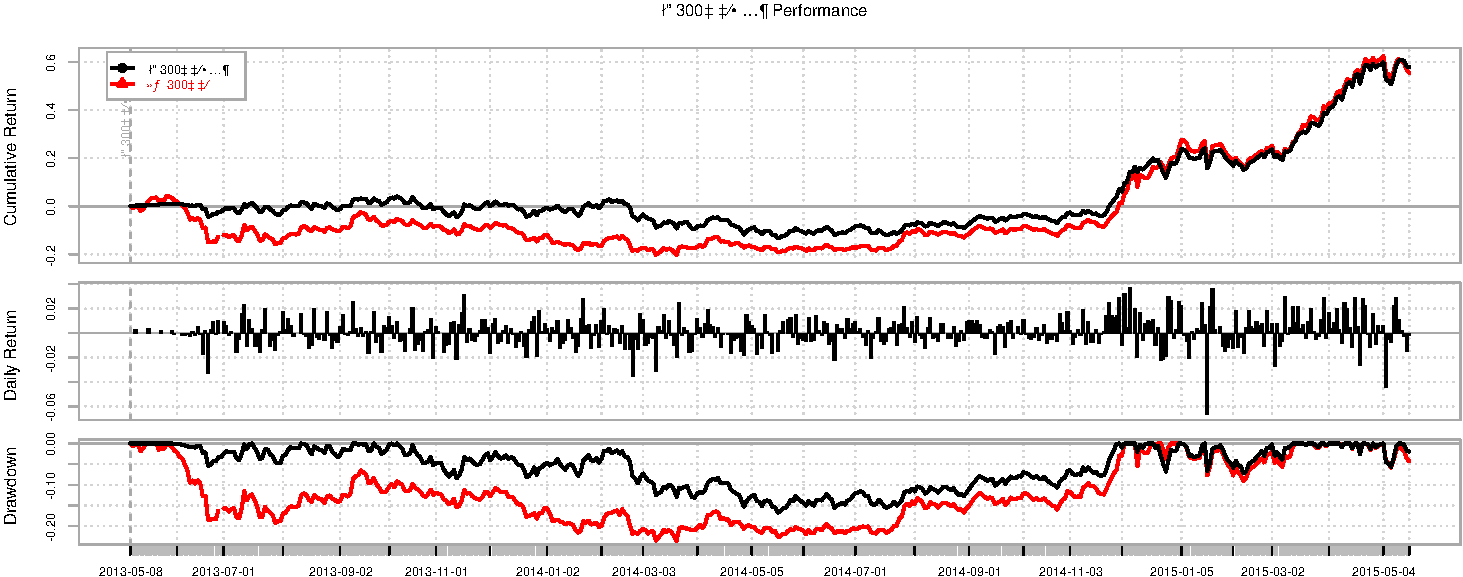
\includegraphics{wangpei-details_files/figure-latex/unnamed-chunk-7-1.pdf}

\begin{longtable}[]{@{}llclclc@{}}
\toprule
名称 & 最后半年 & 夏普率 & 一年 & 夏普率 & 两年 & 夏普率\tabularnewline
\midrule
\endhead
银河300成长分级 & 64\% & 6.2 & 74\% & 1.2 & 58\% & 1.12\tabularnewline
沪深300成长 & 71\% & 6.3 & 87\% & 1.0 & 56\% & 0.93\tabularnewline
\bottomrule
\end{longtable}

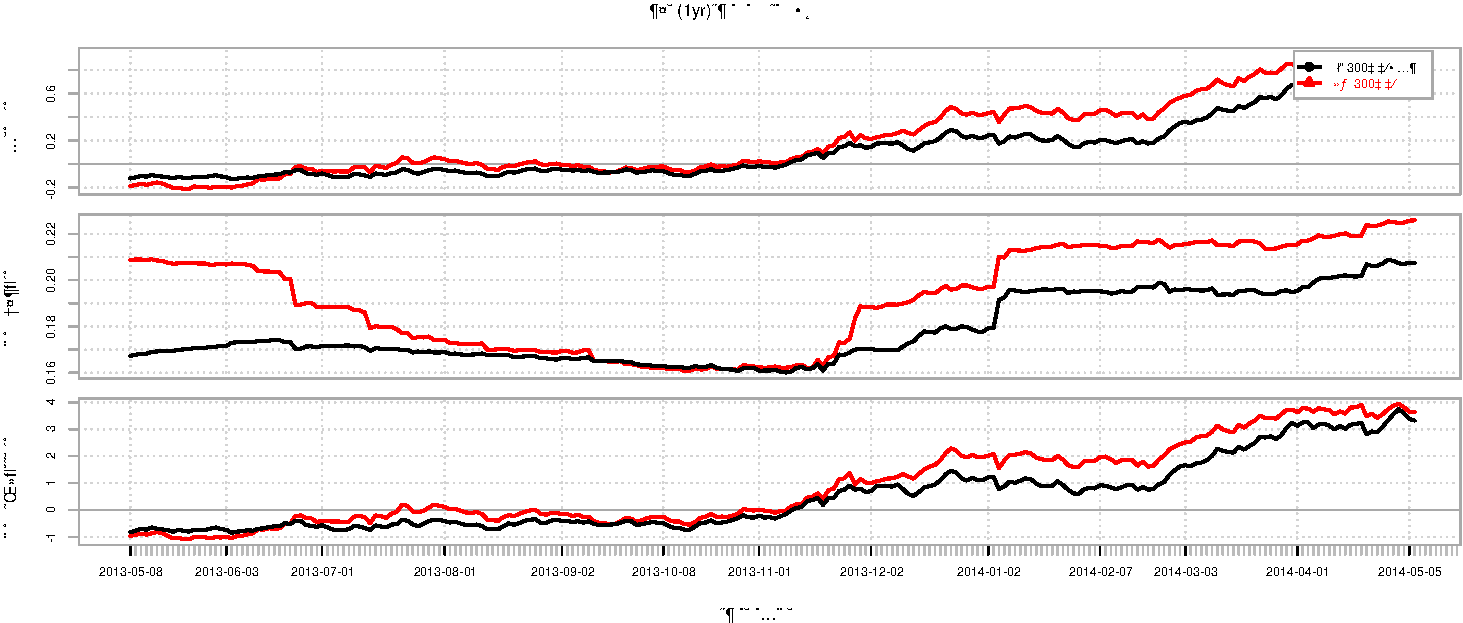
\includegraphics{wangpei-details_files/figure-latex/unnamed-chunk-7-2.pdf}

可以看到,该基金在早期有着比较好的增强效果,后来该增强效果逐渐减弱,进入2014年下半年开始的牛市后,增强基本无效了。

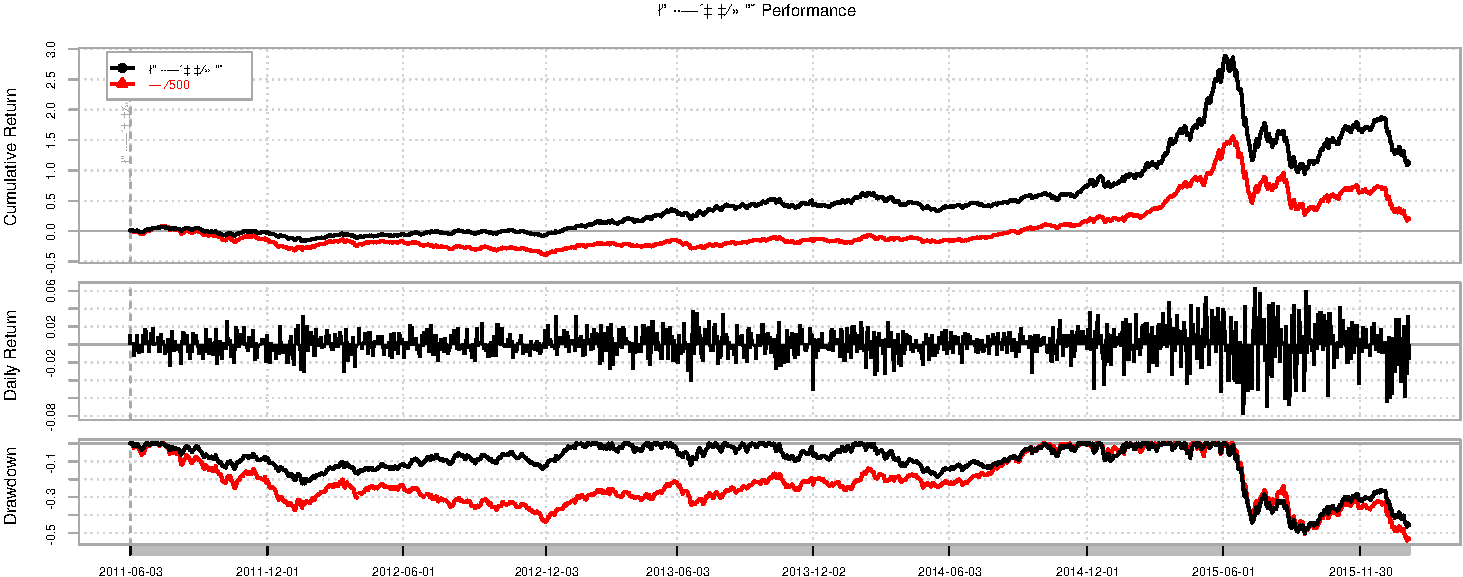
\includegraphics{wangpei-details_files/figure-latex/unnamed-chunk-8-1.pdf}

\begin{longtable}[]{@{}llclclclc@{}}
\toprule
名称 & 最后半年 & 夏普率 & 一年 & 夏普率 & 两年 & 夏普率 & 三年 &
夏普率\tabularnewline
\midrule
\endhead
银河创新成长混合 & -17\% & -0.75 & 15.7\% & 0.27 & 43\% & 0.46 & 117\% &
0.78\tabularnewline
中证500 & -31\% & -1.06 & 2.2\% & -0.02 & 41\% & 0.43 & 81\% &
0.52\tabularnewline
\bottomrule
\end{longtable}

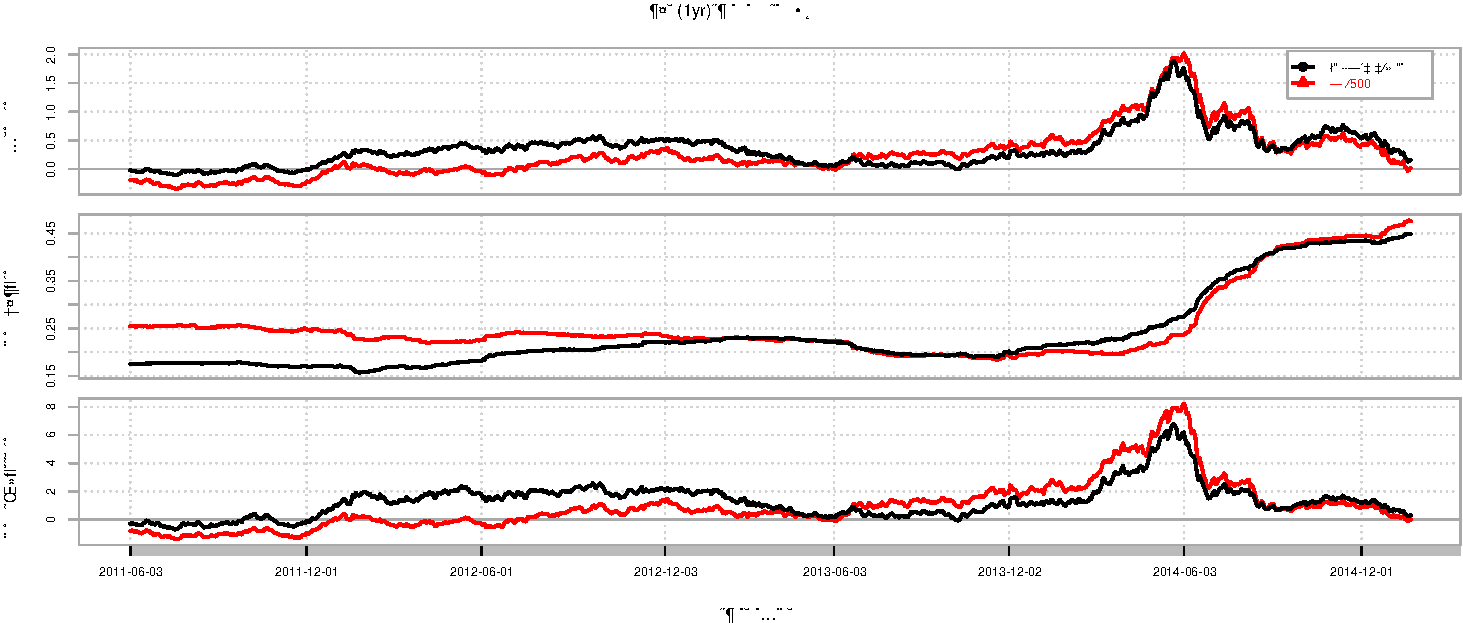
\includegraphics{wangpei-details_files/figure-latex/unnamed-chunk-8-2.pdf}

从上图可以看到,
王培对于投资者的贡献,主要体现在有效的保持与参照指标大致相当的收益率的基础上压缩波动率进而提高风险收益比。

\section{风格分析}

\subsection{交易风格:多变}

在中欧基金管理的中欧行业成长混合展现的风格数据是

\begin{longtable}[]{@{}lcccccc@{}}
\toprule
日期 & 换手率 & 排名\% & 持有期 & 排名\% & 前十占比\% &
排名\%\tabularnewline
\midrule
\endhead
2016 Q2 & 274 & 41 & 0.12 & 84 & 56 & 55\tabularnewline
2016 Q4 & 623 & 36 & 0.06 & 89 & 44 & 75\tabularnewline
\bottomrule
\end{longtable}

\begin{longtable}[]{@{}lccccrcrc@{}}
\toprule
日期 & 行业前5占比\% & 排名\% & 平均集中度 & 排名\% & PE & 排名\% & PB &
排名\%\tabularnewline
\midrule
\endhead
2016 Q2 & 97 & 53 & 0.89 & 14 & 35 & 54 & 4.4 & 42\tabularnewline
2016 Q4 & 95 & 59 & 0.55 & 18 & 28 & 48 & 3.3 & 40\tabularnewline
\bottomrule
\end{longtable}

因为,管理时间还比较短,特征不明显。我们回溯看看历史上王培的交易风格。
基于公开信息,我们对王培在银河成长混合的交易风格分析如下:

\begin{longtable}[]{@{}lcccccc@{}}
\toprule
日期 & 换手率 & 排名\% & 持有期 & 排名\% & 前十占比\% &
排名\%\tabularnewline
\midrule
\endhead
2013 Q4 & 656 & 19 & 0.14 & 63 & 47 & 63\tabularnewline
2014 Q2 & 238 & 30 & 0.21 & 78 & 43 & 74\tabularnewline
2014 Q4 & 632 & 28 & 0.07 & 86 & 62 & 27\tabularnewline
2015 Q2 & 396 & 40 & 0.12 & 73 & 47 & 76\tabularnewline
2015 Q4 & 800 & 49 & 0.05 & 88 & 61 & 44\tabularnewline
\bottomrule
\end{longtable}

\begin{longtable}[]{@{}lccccrcrc@{}}
\toprule
日期 & 行业前5占比\% & 排名\% & 平均集中度 & 排名\% & PE & 排名\% & PB &
排名\%\tabularnewline
\midrule
\endhead
2013 Q4 & 91 & 80 & 0.50 & 42 & 33 & 34 & 5.1 & 25\tabularnewline
2014 Q2 & 96 & 59 & 0.93 & 27 & 24 & 52 & 4.3 & 37\tabularnewline
2014 Q4 & 95 & 41 & 0.68 & 27 & 24 & 48 & 3.6 & 32\tabularnewline
2015 Q2 & 97 & 44 & 0.44 & 39 & 139 & 13 & 15.3 & 3\tabularnewline
2015 Q4 & 90 & 77 & 0.27 & 41 & 29 & 72 & 4.3 & 59\tabularnewline
\bottomrule
\end{longtable}

从以上表格中可以看出该基金的基本交易风格是持股集中度偏高,持股平均PE和PB相对较高,这是成长股的特点。但是需要注意的是在2015年股灾发生后,王培迅速的调整了持有风格转向低PE和低PB的股票,这与股灾后二次、三次触底时,他的基金回撤相对小是有关系的。从中可以看到王培具备一定的学习调整的能力。

同样的对于增强型基金银河300成长分级进行交易风格分析,数据如下:

\begin{longtable}[]{@{}lcccccc@{}}
\toprule
日期 & 换手率 & 排名\% & 持有期 & 排名\% & 前十占比\% &
排名\%\tabularnewline
\midrule
\endhead
2013 Q2 & 243 & 14 & NA & 0 & 47 & 19\tabularnewline
2013 Q4 & 497 & 16 & NA & 0 & 36 & 13\tabularnewline
2014 Q2 & 134 & 34 & 0.38 & 70 & 40 & 16\tabularnewline
2014 Q4 & 475 & 15 & 0.16 & 77 & 40 & 9\tabularnewline
2015 Q2 & 232 & 41 & 0.15 & 88 & 49 & 11\tabularnewline
\bottomrule
\end{longtable}

\begin{longtable}[]{@{}lccccrcrc@{}}
\toprule
日期 & 行业前5占比\% & 排名\% & 平均集中度 & 排名\% & PE & 排名\% & PB &
排名\%\tabularnewline
\midrule
\endhead
2013 Q2 & 91 & 26 & 0.01 & 80 & 7 & 53 & 1.6 & 42\tabularnewline
2013 Q4 & 87 & 58 & 0.00 & 68 & 10 & 41 & 2.2 & 17\tabularnewline
2014 Q2 & 93 & 12 & 0.01 & 54 & 17 & 12 & 3.3 & 9\tabularnewline
2014 Q4 & 88 & 48 & 0.00 & 54 & 9 & 100 & 1.6 & 96\tabularnewline
2015 Q2 & 91 & 27 & 0.00 & 80 & 14 & 44 & 2.5 & 44\tabularnewline
\bottomrule
\end{longtable}

主要特征是交易换手率高,前10占比较大。后者主要由跟踪的指数成分特征来决定,而交易交易换手率高,可以猜测该基金的增强效果是由短线交易获得短时alpha累计而来,随着市场牛市兴起这种频繁交易就显得得不偿失了。

\begin{longtable}[]{@{}lcccccc@{}}
\toprule
日期 & 换手率 & 排名\% & 持有期 & 排名\% & 前十占比\% &
排名\%\tabularnewline
\midrule
\endhead
2011 Q2 & 324 & 10 & NA & 0 & 43 & 61\tabularnewline
2011 Q4 & 548 & 16 & NA & 0 & 57 & 25\tabularnewline
2012 Q2 & 292 & 16 & 0.18 & 86 & 49 & 45\tabularnewline
2012 Q4 & 488 & 22 & 0.11 & 84 & 50 & 42\tabularnewline
2013 Q2 & 368 & 14 & 0.14 & 88 & 48 & 62\tabularnewline
2013 Q4 & 696 & 17 & 0.08 & 88 & 47 & 64\tabularnewline
2014 Q2 & 216 & 33 & 0.24 & 74 & 43 & 74\tabularnewline
2014 Q4 & 667 & 26 & 0.08 & 83 & 59 & 30\tabularnewline
2015 Q2 & 429 & 36 & 0.10 & 82 & 50 & 69\tabularnewline
2015 Q4 & 776 & 51 & 0.05 & 85 & 61 & 44\tabularnewline
\bottomrule
\end{longtable}

\begin{longtable}[]{@{}lccccrcrc@{}}
\toprule
日期 & 行业前5占比\% & 排名\% & 平均集中度 & 排名\% & PE & 排名\% & PB &
排名\%\tabularnewline
\midrule
\endhead
2011 Q2 & 62 & 75 & 0.51 & 50 & 28 & 15 & 3.8 & 48\tabularnewline
2011 Q4 & 80 & 19 & 1.08 & 31 & 25 & 16 & 3.8 & 22\tabularnewline
2012 Q2 & 65 & 68 & 0.10 & 80 & 20 & 42 & 3.3 & 39\tabularnewline
2012 Q4 & 63 & 75 & 0.13 & 68 & 16 & 54 & 2.7 & 44\tabularnewline
2013 Q2 & 86 & 88 & 0.22 & 62 & 47 & 7 & 8.2 & 2\tabularnewline
2013 Q4 & 93 & 64 & 0.51 & 42 & 39 & 20 & 6.3 & 9\tabularnewline
2014 Q2 & 97 & 53 & 0.64 & 37 & 25 & 49 & 4.4 & 36\tabularnewline
2014 Q4 & 97 & 34 & 0.66 & 28 & 17 & 72 & 2.6 & 64\tabularnewline
2015 Q2 & 96 & 49 & 0.37 & 42 & 121 & 18 & 13.6 & 7\tabularnewline
2015 Q4 & 89 & 83 & 0.47 & 29 & 28 & 73 & 4.3 & 59\tabularnewline
\bottomrule
\end{longtable}

在进入中欧基金之前,王培的交易风格的主要特征是多变,不同时期、不同基金产品之间其交易风格都有所不同。\emph{作为基金经理人来说,入行10年,管理基金6年,没有形成自己的风格,要么他是以为灵活多变学习型选手,要么他的投资信念就是跟随市场。}

\subsection{持仓风格:小盘成长到大盘价值}

\subsubsection{中欧行业成长混合}

\begin{longtable}[]{@{}cccc@{}}
\caption{持仓风格权重分析(\%)}\tabularnewline
\toprule
大盘成长 & 大盘价值 & 中盘成长 & 货币\tabularnewline
\midrule
\endfirsthead
\toprule
大盘成长 & 大盘价值 & 中盘成长 & 货币\tabularnewline
\midrule
\endhead
9 & 19 & 67 & 5.1\tabularnewline
\bottomrule
\end{longtable}

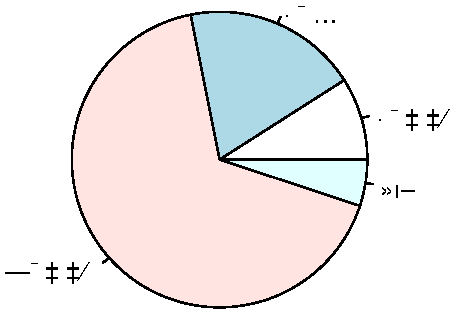
\includegraphics{wangpei-details_files/figure-latex/unnamed-chunk-13-1.pdf}

尽管成长任然是主色调,但是可以看见大盘价值作为第二大因子出现,而且所谓的成长股中,也是配置的大盘或者中盘成长,而不是以前的小盘成长。这是基金经理主动适应市场的变化,是学习型基金管理人的重要标志。

基于净值数据,我们对王培在银河基金中的两支基金的持仓风格分析如下(增强基金由于投资范围的限制,无需分析)。

\subsubsection{银河成长混合}

\begin{longtable}[]{@{}cc@{}}
\caption{持仓风格权重分析(\%)}\tabularnewline
\toprule
小盘成长 & 货币\tabularnewline
\midrule
\endfirsthead
\toprule
小盘成长 & 货币\tabularnewline
\midrule
\endhead
95 & 5\tabularnewline
\bottomrule
\end{longtable}

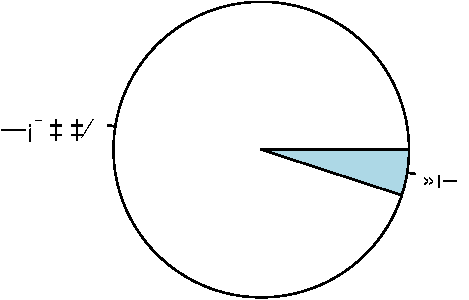
\includegraphics{wangpei-details_files/figure-latex/unnamed-chunk-14-1.pdf}

\subsubsection{银河创新成长混合}

\begin{longtable}[]{@{}ccc@{}}
\caption{持仓风格权重分析(\%)}\tabularnewline
\toprule
小盘成长 & 债券财富指数 & 货币\tabularnewline
\midrule
\endfirsthead
\toprule
小盘成长 & 债券财富指数 & 货币\tabularnewline
\midrule
\endhead
80 & 15 & 5\tabularnewline
\bottomrule
\end{longtable}

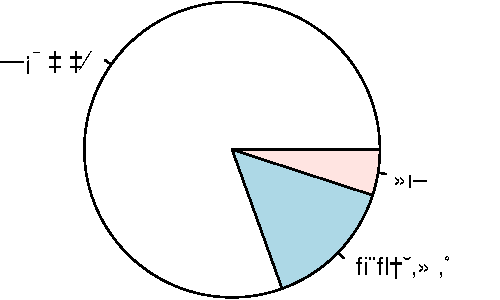
\includegraphics{wangpei-details_files/figure-latex/unnamed-chunk-15-1.pdf}

可见,其重点投资的股票往往都是成长类型的股票。

\subsection{主动风格:积极}

以其管理的银河成长混合为说明,从创建到其接收管理之前,该基金的平均主动管理活跃度为48\%,呈现非常激进的主动管理态势;其接管基金后平均主动管理活跃度为30\%,表现为积极的主动管理。在其管理的同期,整个基金行业的同类型基金的主动管理活跃指数为30\%。因此,\emph{对于王培的管理风格可以定义为积极的主动管理型}

\section{能力评价}

\subsection{大类资产配置:不稳定}

从下图可以看出,在管理期间王培在产品银河成长混合中将股票仓位控制在70-90\%之间,而另外一个产品银河创新成长混合股票仓位则也类似的在70\%-92\%之间变换,显示除了主动的仓位调节。

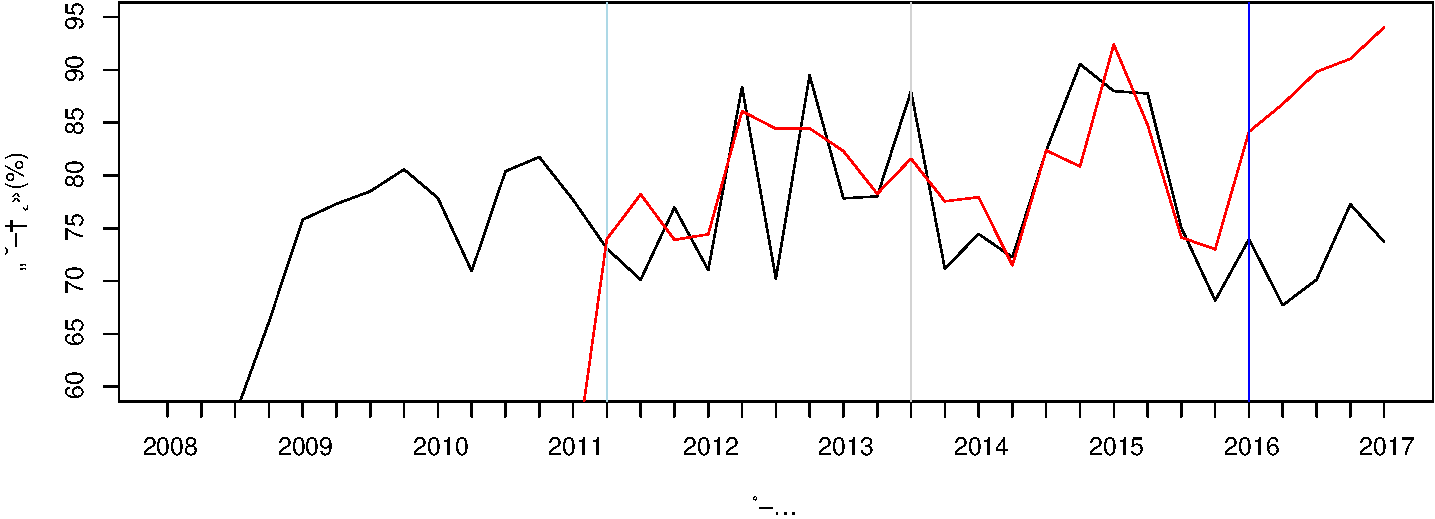
\includegraphics{wangpei-details_files/figure-latex/unnamed-chunk-17-1.pdf}

进一步的计算大类资产配置带来的超额收益。

\subsubsection{中欧行业成长混合}\label{-1}

\begin{longtable}[]{@{}lc@{}}
\caption{银河成长混合大类资产配置能力统计}\tabularnewline
\toprule
日期 & 大类资产配置超额贡献(\%)\tabularnewline
\midrule
\endfirsthead
\toprule
日期 & 大类资产配置超额贡献(\%)\tabularnewline
\midrule
\endhead
2016 Q1 & -0.241\tabularnewline
2016 Q2 & -0.154\tabularnewline
2016 Q3 & -0.093\tabularnewline
2016 Q4 & 0.620\tabularnewline
2017 Q1 & 0.495\tabularnewline
\bottomrule
\end{longtable}

\begin{longtable}[]{@{}cl@{}}
\toprule
平均超额贡献(\%) & 90\%置信区间\tabularnewline
\midrule
\endhead
0.13 & \([-0.15,\infty)\)\tabularnewline
\bottomrule
\end{longtable}

统计显示,在中欧行业成长混合这支基金的管理上,虽然每季度平均取得
0.13\%的配置收益,但是统计意义上还是不显著。

\subsubsection{银河成长混合}\label{-1}

\begin{longtable}[]{@{}lc@{}}
\caption{银河成长混合大类资产配置能力统计}\tabularnewline
\toprule
日期 & 大类资产配置超额贡献(\%)\tabularnewline
\midrule
\endfirsthead
\toprule
日期 & 大类资产配置超额贡献(\%)\tabularnewline
\midrule
\endhead
2013 Q4 & 0.60\tabularnewline
2014 Q1 & 0.39\tabularnewline
2014 Q2 & -0.34\tabularnewline
2014 Q3 & -0.38\tabularnewline
2014 Q4 & 2.50\tabularnewline
2015 Q1 & 1.33\tabularnewline
2015 Q2 & 0.50\tabularnewline
2015 Q3 & -0.60\tabularnewline
2015 Q4 & -1.71\tabularnewline
2016 Q1 & 1.23\tabularnewline
\bottomrule
\end{longtable}

\begin{longtable}[]{@{}cl@{}}
\toprule
平均超额贡献(\%) & 90\%置信区间\tabularnewline
\midrule
\endhead
0.35 & \([-0.16,\infty)\)\tabularnewline
\bottomrule
\end{longtable}

统计显示,在银河成长混合这支基金的管理上,虽然每季度平均取得0.35\%的配置收益,但是统计意义上还是不显著。

\subsubsection{银河创新成长混合}\label{-1}

\begin{longtable}[]{@{}lc@{}}
\caption{银河成长混合大类资产配置能力统计}\tabularnewline
\toprule
日期 & 大类资产配置超额贡献(\%)\tabularnewline
\midrule
\endfirsthead
\toprule
日期 & 大类资产配置超额贡献(\%)\tabularnewline
\midrule
\endhead
2011 Q2 & 0.9817\tabularnewline
2011 Q3 & -0.0029\tabularnewline
2011 Q4 & -0.5414\tabularnewline
2012 Q1 & 0.0828\tabularnewline
2012 Q2 & -0.2194\tabularnewline
2012 Q3 & -0.5652\tabularnewline
2012 Q4 & 0.8950\tabularnewline
2013 Q1 & -0.2696\tabularnewline
2013 Q2 & -0.6656\tabularnewline
2013 Q3 & 0.8042\tabularnewline
2013 Q4 & 0.3893\tabularnewline
2014 Q1 & -0.5112\tabularnewline
2014 Q2 & -0.3849\tabularnewline
2014 Q3 & 0.1672\tabularnewline
2014 Q4 & 2.5791\tabularnewline
2015 Q1 & 1.6553\tabularnewline
2015 Q2 & 1.0045\tabularnewline
2015 Q3 & -1.5155\tabularnewline
2015 Q4 & -0.6376\tabularnewline
2016 Q1 & -0.6014\tabularnewline
\bottomrule
\end{longtable}

\begin{longtable}[]{@{}cl@{}}
\toprule
平均超额贡献\% & 90\%置信区间\tabularnewline
\midrule
\endhead
0.13 & \([-0.15,\infty)\)\tabularnewline
\bottomrule
\end{longtable}

统计显示,在银河创新成长混合这支基金的管理上,每季度平均取得
0.13\%的配置收益,
统计意义上也不显著。因此王培并没有显示出稳健的大类资产配置的能力。

\subsection{行业配置能力:弱}

既然基金产品的超额收益并非得益于大类资产的配置,那么比如来自与行业配置、选股以及择时的能力。需要提前指出的是,这三个能力在逻辑与实践中都不是相互独立的。好的投资标的往往也意味着好的投资时机,而好股票的挖掘与选择自然也带来了相应行业的配置偏好。但是这三种能力又在某种程度上可以区别开来,因为它们毕竟是在投资的不同决策层面和时点上的投资活动。我们认为:

\begin{longtable}[]{@{}lll@{}}
\toprule
行为 & 动机 & 度量方法\tabularnewline
\midrule
\endhead
行业配置 & smart beta & \(\sum(w_i-w_i^B)(r_i^B-r^B)\)\tabularnewline
择股 & 持续的alpha & \(\sum w_{i}(r_{i}^F-r_{i}^B)\)\tabularnewline
择时 & 动态的alpha & 未解释的差额部分\tabularnewline
\bottomrule
\end{longtable}

因为所获得数据精确程度的不同,我们计算的以上三个方面能力对于总超额收益的贡献比例可能是不精确的,读者应该更多的关注其相对值以及相关的统计推论。

\begin{longtable}[]{@{}lcc@{}}
\caption{中欧行业成长混合行业配置能力}\tabularnewline
\toprule
日期 & 行业配置成功率\% & 行业配置贡献超额收益率\%\tabularnewline
\midrule
\endfirsthead
\toprule
日期 & 行业配置成功率\% & 行业配置贡献超额收益率\%\tabularnewline
\midrule
\endhead
2016 Q1 & 14 & -1.62\tabularnewline
2016 Q2 & -12 & 0.06\tabularnewline
2016 Q4 & 10 & 0.60\tabularnewline
2017 Q1 & 20 & 0.55\tabularnewline
\bottomrule
\end{longtable}

\begin{longtable}[]{@{}cl@{}}
\toprule
平均超额贡献\% & 90\%置信区间\tabularnewline
\midrule
\endhead
-0.1 & \([-0.95,\infty)\)\tabularnewline
\bottomrule
\end{longtable}

从统计结果可以看出,王培在中欧行业成长混合基金的管理上没有显示行业配置能力,平均超额表现为-0.1\%每半年,年化-0.4\%。

\begin{longtable}[]{@{}lcc@{}}
\caption{银河成长混合行业配置能力}\tabularnewline
\toprule
日期 & 行业配置成功率\% & 行业配置贡献超额收益率\%\tabularnewline
\midrule
\endfirsthead
\toprule
日期 & 行业配置成功率\% & 行业配置贡献超额收益率\%\tabularnewline
\midrule
\endhead
2013 Q4 & 11 & -0.37\tabularnewline
2014 Q1 & 11 & 0.89\tabularnewline
2014 Q2 & 10 & 2.02\tabularnewline
2014 Q3 & 10 & 2.76\tabularnewline
2014 Q4 & -14 & -17.86\tabularnewline
2015 Q1 & 14 & 24.57\tabularnewline
2015 Q2 & -14 & -1.31\tabularnewline
2015 Q4 & -14 & 4.35\tabularnewline
2016 Q1 & -12 & -2.50\tabularnewline
\bottomrule
\end{longtable}

\begin{longtable}[]{@{}cl@{}}
\toprule
平均超额贡献\% & 90\%置信区间\tabularnewline
\midrule
\endhead
1.4 & \([-3.67,\infty)\)\tabularnewline
\bottomrule
\end{longtable}

从统计结果可以看出,王培在银河成长混合基金的管理上显示了一定的行业配置能力,平均超额表现为1.39\%每半年,年化5.7\%。但是波动较大,统计不显著。

\begin{longtable}[]{@{}lcc@{}}
\caption{银河300成长分级行业配置能力}\tabularnewline
\toprule
日期 & 行业配置成功率\% & 行业配置贡献超额收益率\%\tabularnewline
\midrule
\endfirsthead
\toprule
日期 & 行业配置成功率\% & 行业配置贡献超额收益率\%\tabularnewline
\midrule
\endhead
2013 Q2 & 9.1 & 0.84\tabularnewline
2013 Q3 & 9.1 & 0.84\tabularnewline
2013 Q4 & 7.7 & -0.24\tabularnewline
2014 Q1 & -9.1 & 0.92\tabularnewline
2014 Q2 & 10.0 & 1.50\tabularnewline
2014 Q3 & 10.0 & -0.07\tabularnewline
2014 Q4 & 7.7 & 7.76\tabularnewline
2015 Q1 & -8.3 & -1.09\tabularnewline
2015 Q2 & 9.1 & -1.96\tabularnewline
\bottomrule
\end{longtable}

\begin{longtable}[]{@{}cl@{}}
\toprule
平均超额贡献\% & 90\%置信区间\tabularnewline
\midrule
\endhead
0.94 & \([-0.35,\infty)\)\tabularnewline
\bottomrule
\end{longtable}

从统计结果可以看出,王培在银河300成长分级基金的管理上显示了一定的行业配置能力,平均超额表现为0.94\%每半年,年化3.83\%。

\begin{longtable}[]{@{}lcc@{}}
\caption{银河创新成长混合行业配置能力}\tabularnewline
\toprule
日期 & 行业配置成功率\% & 行业配置贡献超额收益率\%\tabularnewline
\midrule
\endfirsthead
\toprule
日期 & 行业配置成功率\% & 行业配置贡献超额收益率\%\tabularnewline
\midrule
\endhead
2011 Q2 & 12.5 & -1.46\tabularnewline
2011 Q3 & 7.1 & 4.96\tabularnewline
2011 Q4 & 8.3 & -0.17\tabularnewline
2012 Q1 & 6.7 & -14.29\tabularnewline
2012 Q2 & 6.2 & 4.22\tabularnewline
2012 Q3 & -7.7 & -0.44\tabularnewline
2012 Q4 & 7.1 & -3.49\tabularnewline
2013 Q1 & 10.0 & 1.97\tabularnewline
2013 Q2 & -7.7 & 4.10\tabularnewline
2013 Q3 & 9.1 & 11.89\tabularnewline
2013 Q4 & 9.1 & -0.40\tabularnewline
2014 Q1 & 10.0 & 1.02\tabularnewline
2014 Q2 & 10.0 & 2.02\tabularnewline
2014 Q3 & 9.1 & 2.55\tabularnewline
2014 Q4 & -14.3 & -13.68\tabularnewline
2015 Q1 & 7.7 & 17.78\tabularnewline
2015 Q2 & 11.1 & -0.23\tabularnewline
2015 Q4 & -11.1 & 3.99\tabularnewline
2016 Q1 & -12.5 & -1.68\tabularnewline
\bottomrule
\end{longtable}

\begin{longtable}[]{@{}cl@{}}
\toprule
平均超额贡献\% & 90\%置信区间\tabularnewline
\midrule
\endhead
0.98 & \([-1.22,\infty)\)\tabularnewline
\bottomrule
\end{longtable}

从统计结果可以看出,王培在银河创新成长混合基金的管理上显示了一定的行业配置能力,平均超额表现为0.98\%每半年,年化3.99\%。

\subsection{择股能力:比较强!}

公开渠道获得的持仓数据频率为每半年一次。我们依据此数据分析基金管理人的择股能力。当然,由于更新频率粗糙,读者有理由担心计算精度的问题。不过从另外一个角度看,我们所谓的择股能力是对照于择时能力而言获取相对持续的alpha的能力。这里的相对持续,完全可以根据我们研究的需要而定义。此处,定义半年为一个相对持续的alpha的标准,也是合情合理的。当前受制于数据不完整,此项能力分析最早只能回溯到2013年。

\begin{longtable}[]{@{}lcc@{}}
\caption{中欧行业成长混合择股能力}\tabularnewline
\toprule
日期 & 行业择股成功率\% & 择股贡献超额收益率\%\tabularnewline
\midrule
\endfirsthead
\toprule
日期 & 行业择股成功率\% & 择股贡献超额收益率\%\tabularnewline
\midrule
\endhead
2016 Q1-2 & 9.1 & 10.15\tabularnewline
2016 Q3-4 & -9.1 & 2.43\tabularnewline
2017 Q1-2 & 10.0 & 15.15\tabularnewline
2017 Q3-4 & 50.0 & 0.92\tabularnewline
\bottomrule
\end{longtable}

\begin{longtable}[]{@{}cl@{}}
\toprule
平均超额贡献\% & 90\%置信区间\tabularnewline
\midrule
\endhead
7.2 & \([1.69,\infty)\)\tabularnewline
\bottomrule
\end{longtable}

从统计结果可以看出,王培在中欧行业成长混合基金的管理上显示了明显的择股能力------即他能够选择出在未来6个月的投资周期上回报好于对应行业指数表现的股票组合,而且择股能力贡献的平均超额表现高达7.16\%每半年,年化14.84\%。

\begin{longtable}[]{@{}lcc@{}}
\caption{银河成长混合择股能力}\tabularnewline
\toprule
日期 & 行业择股成功率\% & 择股贡献超额收益率\%\tabularnewline
\midrule
\endfirsthead
\toprule
日期 & 行业择股成功率\% & 择股贡献超额收益率\%\tabularnewline
\midrule
\endhead
2013 Q3-4 & 9.1 & 13\tabularnewline
2014 Q1-2 & -8.3 & 4\tabularnewline
2014 Q3-4 & -9.1 & 16\tabularnewline
2015 Q1-2 & 9.1 & 115\tabularnewline
2015 Q3-4 & 11.1 & 20\tabularnewline
2016 Q1-2 & 7.7 & 13\tabularnewline
\bottomrule
\end{longtable}

\begin{longtable}[]{@{}cl@{}}
\toprule
平均超额贡献\% & 90\%置信区间\tabularnewline
\midrule
\endhead
30 & \([5.05,\infty)\)\tabularnewline
\bottomrule
\end{longtable}

从统计结果可以看出,王培在银河成长混合基金的管理上显示了明显的择股能力------即他能够选择出在未来6个月的投资周期上回报好于对应行业指数表现的股票组合,而且择股能力贡献的平均超额表现高达30.32\%每半年,年化69.84\%。

\begin{longtable}[]{@{}lcc@{}}
\caption{银河300成长分级择股能力}\tabularnewline
\toprule
日期 & 行业择股成功率\% & 择股贡献超额收益率\%\tabularnewline
\midrule
\endfirsthead
\toprule
日期 & 行业择股成功率\% & 择股贡献超额收益率\%\tabularnewline
\midrule
\endhead
2013 Q1-2 & 9.1 & 5.7\tabularnewline
2013 Q3-4 & 7.1 & 4.9\tabularnewline
2014 Q1-2 & -7.1 & -5.9\tabularnewline
2014 Q3-4 & 6.7 & 21.6\tabularnewline
2015 Q1-2 & -7.7 & 16.6\tabularnewline
\bottomrule
\end{longtable}

\begin{longtable}[]{@{}cl@{}}
\toprule
平均超额贡献\% & 90\%置信区间\tabularnewline
\midrule
\endhead
8.6 & \([1.19,\infty)\)\tabularnewline
\bottomrule
\end{longtable}

从统计结果可以看出,王培在银河300成长分级基金的管理上显示了明显的择股能力------即他能够选择出在未来6个月的投资周期上回报好于对应行业指数表现的股票组合,而且择股能力贡献的平均超额表现高达8.58\%每半年,年化17.9\%。须知这是在沪深300成长指数成分股和备选股中选择的股票,能够有这样的表现实属不易。

\begin{longtable}[]{@{}lcc@{}}
\caption{银河创新成长混合择股能力}\tabularnewline
\toprule
日期 & 行业择股成功率\% & 择股贡献超额收益率\%\tabularnewline
\midrule
\endfirsthead
\toprule
日期 & 行业择股成功率\% & 择股贡献超额收益率\%\tabularnewline
\midrule
\endhead
2013 Q1-2 & 8.3 & 35.8\tabularnewline
2013 Q3-4 & 8.3 & 12.0\tabularnewline
2014 Q1-2 & -9.1 & 4.6\tabularnewline
2014 Q3-4 & -9.1 & 17.1\tabularnewline
2015 Q1-2 & 9.1 & 79.4\tabularnewline
2015 Q3-4 & -9.1 & 21.0\tabularnewline
2016 Q1-2 & 8.3 & 12.4\tabularnewline
\bottomrule
\end{longtable}

\begin{longtable}[]{@{}cl@{}}
\toprule
平均超额贡献\% & 90\%置信区间\tabularnewline
\midrule
\endhead
26 & \([12.19,\infty)\)\tabularnewline
\bottomrule
\end{longtable}

从统计结果可以看出,王培在银河创新成长混合基金的管理上显示了明显的择股能力------即他能够选择出在未来6个月的投资周期上回报好于对应行业指数表现的股票组合,而且择股能力贡献的平均超额表现高达26.06\%每半年,年化58.9\%。

当然,我们也需要客观的指出,王培的超强的择股能力的一部分贡献,来自与2015年上半年,他在多只基金中的亮眼表现。尽管我们在计算择股能力的时候,使用的是超额收益,即减去参照指标(一般是沪深300指数)后的超出部分。按理已经排除了牛市的影响,将其完全归集为择股能力并无问题。但是需要指出,中国市场的问题很多,尤其牛市期间,``妖股''频出。这些不可言状的``妖股'',也许成就了基金经理人的辉煌人生,不无不可,毕竟``人脉''或者``运气''也是能力的一部分。但就以此建立一个择股能力的最高标杆,则误导大众了。因此可以考虑将这段时间的数据排除出去进行分析。那样的话,我们得出王培的择股能力也是比较强的(当然,不再是超强)。

\subsection{择时能力:灾难性}

择时能力在本文的设定中包括以下方面:

\begin{itemize}
\tightlist
\item
  交易周期短于半年的动态alpha机会,如一些短期事件性投资机会、相对明确的业绩反转预期等。
\item
  上升通道中的止盈能力
\item
  下降通道中的止亏能力
\end{itemize}

所以择时能力并不总是能够带来正的超额收益,但是它能够确保落袋为安(止盈能力)或者保命再战(止亏能力),对于提高基金的风险收益比(如夏普率)是十分重要的。

\begin{longtable}[]{@{}lc@{}}
\caption{中欧行业成长混合择时能力}\tabularnewline
\toprule
日期 & 择时能力贡献超额收益率\%\tabularnewline
\midrule
\endfirsthead
\toprule
日期 & 择时能力贡献超额收益率\%\tabularnewline
\midrule
\endhead
2016 Q1-2 & -14.3\tabularnewline
2016 Q3-4 & -6.6\tabularnewline
2017 Q1-2 & -6.6\tabularnewline
\bottomrule
\end{longtable}

\begin{longtable}[]{@{}cl@{}}
\toprule
平均超额贡献\% & 90\%置信区间\tabularnewline
\midrule
\endhead
-9.2 & \([-14.06,\infty)\)\tabularnewline
\bottomrule
\end{longtable}

从上表中可以看出,王培在中欧行业成长混合基金的管理上显示了明显的负的择时能力,而且择时能力贡献的平均超额表现多达-9.19\%每半年,年化-17.53\%。

\begin{longtable}[]{@{}lc@{}}
\caption{银河成长混合择时能力}\tabularnewline
\toprule
日期 & 择时能力贡献超额收益率\%\tabularnewline
\midrule
\endfirsthead
\toprule
日期 & 择时能力贡献超额收益率\%\tabularnewline
\midrule
\endhead
2013 Q3-4 & -23.7\tabularnewline
2014 Q1-2 & -12.3\tabularnewline
2014 Q3-4 & -12.6\tabularnewline
2015 Q1-2 & -61.8\tabularnewline
2015 Q3-4 & -6.2\tabularnewline
2016 Q1-2 & -31.5\tabularnewline
\bottomrule
\end{longtable}

\begin{longtable}[]{@{}cl@{}}
\toprule
平均超额贡献\% & 90\%置信区间\tabularnewline
\midrule
\endhead
-25 & \([-36.95,\infty)\)\tabularnewline
\bottomrule
\end{longtable}

从上表中可以看出,王培在银河成长混合基金的管理上显示了明显的负的择时能力,而且择时能力贡献的平均超额表现多达-24.7\%每半年,年化-43.31\%。

\begin{longtable}[]{@{}lc@{}}
\caption{银河300成长分级择时能力}\tabularnewline
\toprule
日期 & 择时能力贡献超额收益率\%\tabularnewline
\midrule
\endfirsthead
\toprule
日期 & 择时能力贡献超额收益率\%\tabularnewline
\midrule
\endhead
2013 Q1-2 & -11.62\tabularnewline
2013 Q3-4 & -8.77\tabularnewline
2014 Q1-2 & -4.55\tabularnewline
2014 Q3-4 & -8.20\tabularnewline
2015 Q1-2 & -0.05\tabularnewline
\bottomrule
\end{longtable}

\begin{longtable}[]{@{}cl@{}}
\toprule
平均超额贡献\% & 90\%置信区间\tabularnewline
\midrule
\endhead
-6.6 & \([-9.70,\infty)\)\tabularnewline
\bottomrule
\end{longtable}

从上表中可以看出,王培在银河300成长分级基金的管理上显示了明显的负的择时能力,而且择时能力贡献的平均超额表现多达-6.64\%每半年,年化-12.84\%。

\begin{longtable}[]{@{}lc@{}}
\caption{银河创新成长混合择时能力}\tabularnewline
\toprule
日期 & 择时能力贡献超额收益率\%\tabularnewline
\midrule
\endfirsthead
\toprule
日期 & 择时能力贡献超额收益率\%\tabularnewline
\midrule
\endhead
2013 Q1-2 & -14.8\tabularnewline
2013 Q3-4 & 2.7\tabularnewline
2014 Q1-2 & -8.9\tabularnewline
2014 Q3-4 & -10.6\tabularnewline
2015 Q1-2 & -41.3\tabularnewline
2015 Q3-4 & -4.6\tabularnewline
2016 Q1-2 & -27.0\tabularnewline
\bottomrule
\end{longtable}

\begin{longtable}[]{@{}cl@{}}
\toprule
平均超额贡献\% & 90\%置信区间\tabularnewline
\midrule
\endhead
-15 & \([-22.97,\infty)\)\tabularnewline
\bottomrule
\end{longtable}

从上表中可以看出,王培在银河创新成长混合基金的管理上显示了不太显著的的择时能力,而且择时能力贡献的平均超额表现为-14.92\%每半年,年化-27.62\%。

综上,我们认为王培作为一名风格多变的成长股投资者,他在择时能力上的表现是灾难性的。减少追涨杀跌或者增加持股时间或可带来表现上的改变。

\section{投资方法体系}

\subsection{成长股精选}

\begin{itemize}
\item 将成长股的概念推广到,扩张到周期性、消费性行业等,实际上是将自己熟悉的成长股的研究方法进行推广:
\begin{itemize}
  \item 稳定增长类:以基本面投资为主;
  \item 周期类:以趋势投资为主;
  \item 阶段高成长类:主题投资为主。
  \end{itemize}
\item 寻找低估值资产和预期差:
\begin{itemize}
  \item 低估值资产是决定是否投资的关键;
  \item 预期差决定买入卖出的时点。
\end{itemize}

\end{itemize}

\subsection{风控方法}

\begin{itemize}
\tightlist
\item
  不断衡量个股估计阶段性业绩与风格表现是否匹配来加减仓位;
\item
  行业配置调整避免过高集中度;
\item
  避免估值陷阱,即使估值很便宜但在基本面变差时也要及时卖出。
\end{itemize}

\section{评价}

王培是既往的成长股明星,在市场风格转变之后,经历过一段艰难转型,走向成长价值的方向上。我们基于公开信息,进行深度的科学分析,结合与其面对面的交流,做出如下评判:

\begin{enumerate}
\def\labelenumi{\arabic{enumi}.}
\tightlist
\item
  王培的交易风格不明确,甚至可以说过于频繁的操作带来了不必要的收益损失;
\item
  王培的持仓风格有从小盘成长,往大盘价值和大中盘成长转变的明确历程,深刻说明他是一位有适应能力的学习型的基金管理人,但是他的转变与继承是否能够超越市场回到他从前的高度还需要时间的验证;
\item
  作为一名``自下而上''的投资人,在大类资产配置和行业配置能力没有太出色的表现;
\item
  作为前期典型的成长股投资者和现在转型的成长价值投资这,择股能力是最为重要的盈利手段之一,王培在该项目上表现了持续有效的能力。
\end{enumerate}

因此,王培是适应多种市场风格、擅长成长类投资、积极主动的基金管理人。

\end{document}
